\subsubsection{External interfaces}

\begin{figure}[h]
	\centering
	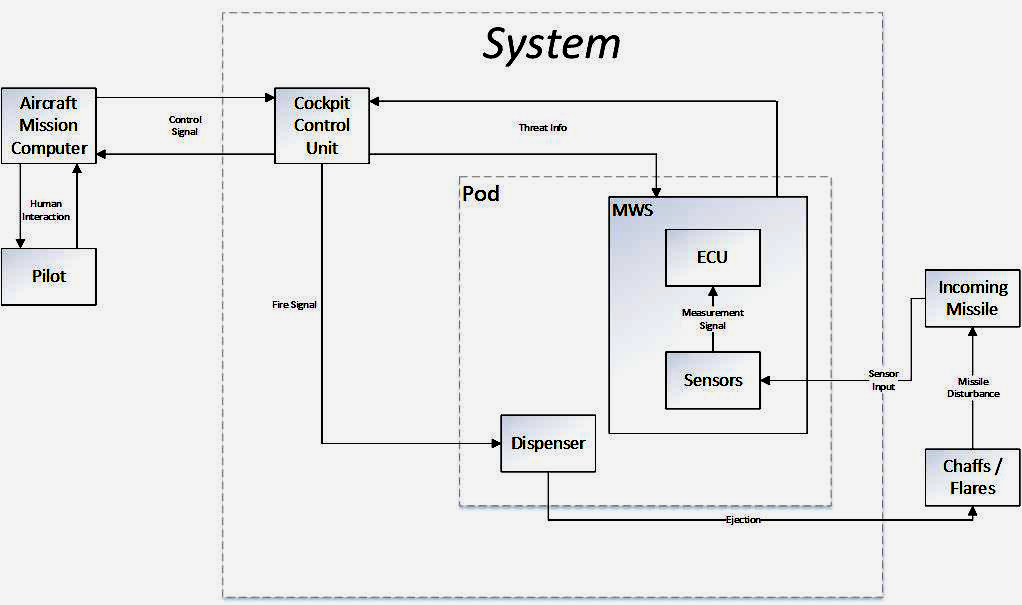
\includegraphics[scale=0.5]{./images/SignalFlowDiagram}\\
	\caption{Signal Flow Diagram}
    \label{fig:sigFlowDiagram}
\end{figure}
\begin{itemize}
\item {Interface identification and diagrams.}\\
blaa
\item {Project-unique identifier of interface}\\
blaa
\end{itemize}

\subsubsection{Internal interfaces}
This section describes the internal interfaces. The system interfaces can be seen on figure \ref{fig:sigOverviewIdentification}. The internal interfaces are:

\begin{itemize}
\item I-IF-MWSCTRL
\item I-IF-DISCTRL
\end{itemize}

\paragraph{I-IF-MWSCTRL}

\begin{center}
\begin{tabular}{ | p{2cm} | l | p{1.6cm} | p{1.6cm} | l | p{1cm} |}
\hline
 \textbf{Interface name} & \textbf{Identification} & \textbf{Endpoint A} & \textbf{Endpoint B} & \textbf{Standard}\\ \hline

 MWS Control & I-IF-MWSCTRL & Cockpit unit & MWS & MIL-STD-1553-B\\ \hline

\end{tabular}
\end{center}

Some description...
\\
Something about data:
\begin{itemize}
\item Threat data
	\begin{itemize}
	\item direction
	\item type
	\item velocity
	\end{itemize}
\end{itemize}
The physical layer is defined by the MIL-STD-1553-B standard.


\paragraph{I-IF-DISCTRL}

\begin{center}
\begin{tabular}{ | p{2cm} | l | p{1.6cm} | p{1.6cm} | l | p{1cm} |}
\hline
 \textbf{Interface name} & \textbf{Identification} & \textbf{Endpoint A} & \textbf{Endpoint B} & \textbf{Standard}\\ \hline

 Dispenser Control & IF-DISCTRL & Cockpit unit & Dispenser assembly & MIL-STD-1553-B\\ \hline
 
\end{tabular}
\end{center}

Some description...\\
Something about data:
\begin{itemize}
\item direction to fire
\item what to fire (chaffs/flares)
\item pattern to fire
\item fire command
\end{itemize}

The physical layer is defined by the MIL-STD-1553-B standard.